\chapter{Communities in primate and human societies}
\label{ch:societies}

\section{Locality or likeness?}

Chapter~\ref{ch:communities} showed that a network grown by a local rule partitions
itself. No node in $LS(n,1)$ or $DS(n,q)$ differs from any other, yet above the Ramsey
community number $r_\kappa$ the block model finds communities with near certainty. The
communities record the history of the growth, not the properties of the nodes.

The social sciences have a different and older explanation for the same observation:
\emph{homophily}, the tendency of similar individuals to bond \citep{mcpherson2001}.
On that view a community is the visible trace of something its members share ---
kinship, language, status, belief --- and the explanation has been projected into deep
time. Models of cultural evolution propose that marking group identity with arbitrary
symbols became adaptive because it let individuals find partners with compatible norms
\citep{mcelreath2003}, which makes homophily a founding force of early human social
structure. Those models are hypotheses about the past. The question this chapter asks is
what the record of primate and human societies says, and it treats neither mechanism as
the default.

The question is sharper than it looks, because the two mechanisms share their
ingredients. Real ties form through friends of friends, the kin of kin, the neighbors of
neighbors: these are local rules, and Chapter~\ref{ch:friends} built the friend of a
friend into a growth model with clustering and assortativity
\citep{jin2001,vazquez2003,toivonen2006}. And $r_\kappa$, measured at $81$ for
$LS(n,1)$ and $98$ for $DS(n,0.5)$ with the block model of
Chapter~\ref{ch:communities}, sits at the scale of forager
bands, primate communities and early villages. If local growth builds communities at
all, these are the sizes at which it should begin to show.

Three obstacles stand between that prediction and a test. In a single snapshot,
homophily (similar individuals bond) and contagion (bonded individuals become similar)
produce the same correlation between ties and traits \citep{shalizi2011}. Space mimics
both, since neighbors meet more often and also resemble each other. And the most
important trait in a small-scale society, kinship, is itself a network: a genealogy,
grown by descent and marriage, which are local rules. The chapter therefore proceeds in
two steps. It first grows synthetic societies in which the share of homophily is known
and asks which statistics recover it at the sizes of real groups. It then applies the
statistics that work to four records: the fission of a chimpanzee community, support
networks in two small-scale human societies, kinship networks from ancient genomes, and
three centuries of ceramic exchange in the North American Southwest.

\section{What a small society can reveal}

The synthetic societies mix the two mechanisms with one knob. Growth adds a node with two
links per step. In $LS(n,1)$ the first link goes to a uniformly chosen anchor and the
second to a random neighbor of the anchor; in $DS(n,0.5)$ the newcomer copies and splits
the links of an existing node. Each node carries one of $K=2$ balanced types, and a share
$\lambda$ of links (in $LS$) or of newcomers (in $DS$) is placed instead by homophily:
with probability $h=0.8$ the target is restricted to the newcomer's type and chosen in
proportion to degree plus one \citep{karimi2018}. Thus $\lambda=0$ is pure locality,
$\lambda=1$ is pure homophily, and the degree distribution barely moves between them, so
the knob changes where links go and not how many each node gets. The controls are a
static block model on the types, a spatial model in which links decay with distance and
type is set by position, and the Barab\'asi--Albert model of
Chapter~\ref{ch:communities}. In the contagion variant two nodes per step copy a
neighbor's type with probability $1-\lambda$, so that a society grown by locality
acquires its trait correlations afterwards. Sizes run from $n=20$ to $n=500$, with $60$
replicates per condition and $15\,260$ networks in all.

Each candidate statistic is scored by its power to separate $\lambda=0$ from $\lambda=1$,
measured as the area under the receiver operating characteristic curve (AUC): $1$ is
perfect, $0.5$ is chance, and below $0.5$ the statistic points the wrong way. Three
results organize everything that follows.

\begin{figure}[!ht]
\centering
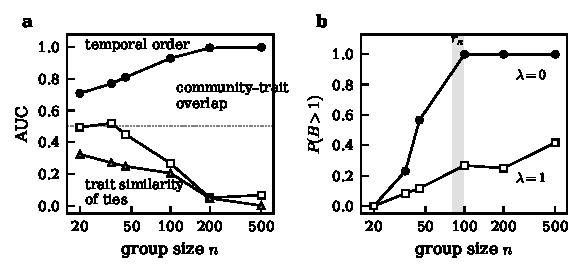
\includegraphics[width=\linewidth]{figs/fig-soc-power.pdf}
\caption{\textbf{What a small society can reveal.} (a) Power (AUC) to separate locality
($\lambda=0$) from homophily ($\lambda=1$) when traits also spread along ties, against
group size $n$. Snapshot statistics --- the similarity of tied individuals, and the
overlap of block-model communities with the trait --- fall below chance; the temporal
statistic, similarity gained after a tie forms, rises towards $1$. Dotted line, chance.
(b) Probability $P(B>1)$ that the block model finds more than one community, for
$LS(n,1)$ at $\lambda=0$ and $\lambda=1$. The gray band marks $r_\kappa$. $60$
replicates per point.}
\label{fig:soc-power}
\end{figure}

\paragraph{Tests that take the trait as given are powerful.} A dyadic logistic model of
ties on shared trait, common neighbors, log degrees and distance separates the two worlds
with AUC $\ge0.99$ already at $n=20$, and its coefficients recover $\lambda$. The model
asks whether the trait predicts ties beyond what the network's own structure predicts,
and the network's own structure is exactly what locality leaves behind.

\paragraph{Tests that first infer communities are weak.} Comparing block-model
communities with the trait has little power at any size
(Fig.~\ref{fig:soc-power}b). Below $r_\kappa$ the locally grown societies have no
detectable communities, as Chapter~\ref{ch:communities} predicts. The homophilous
societies are worse off: their blocks never become reliably detectable, at any size. The
reason is an information threshold, and it does not depend on $n$.

\begin{calculation}{when homophily blocks can be seen}
Let $K$ balanced types carry a fraction $p$ of the edges within types, with mean degree
$\langle k\rangle$. Labeling the nodes by type saves, per edge, the Kullback--Leibler
divergence between the observed placement of edges and the placement without types,
\begin{equation}
  D(p,K) = p\ln(pK) + (1-p)\ln\frac{(1-p)K}{K-1},
  \label{eq:soc-kl}
\end{equation}
since a random edge falls within a type with probability $1/K$. With $m=n\langle
k\rangle/2$ edges the description of the network shortens by $mD$, while the labels
themselves cost $n\ln K$. The block partition pays for itself only if $mD>n\ln K$, that is
\begin{equation}
  \frac{\langle k\rangle}{2}\,D(p,K) > \ln K .
  \label{eq:soc-detect}
\end{equation}
The size $n$ has cancelled. A homophilous society of given density and given strength of
homophily is either above the threshold at every size or below it at every size. For the
synthetic societies, $K=2$ and $p=0.9$ give $D=0.37$, so the left side of
Eq.~\eqref{eq:soc-detect} at $\langle k\rangle=4$ is $0.74$, barely above $\ln 2=0.69$.
The blocks sit at the detection limit, and finite-size fluctuations keep $P(B>1)$ well
below $1$.
\end{calculation}

The practical consequence is that the absence of communities in a group of fifty says
nothing about mechanism. Locality predicts none at that size, and homophily at realistic
density predicts few at any size.

\paragraph{Contagion reverses every snapshot.} When traits spread along ties, a society
grown by locality acquires trait correlations that are stronger and more regular than
those of a truly homophilous society, because contagion copies the trait along every tie
while homophily places only some ties by it. Every snapshot statistic built on the trait
then points the wrong way, with AUC falling towards zero as $n$ grows
(Fig.~\ref{fig:soc-power}a). Only the temporal order survives: whether similarity follows
a tie or precedes it. This is the confound of \citet{shalizi2011} measured at the sizes
where it matters, and it fixes the design of what follows. A snapshot can rule out a
measured trait as the organizer of a network. It cannot decide between locality and
contagion, or between locality and homophily on a trait nobody measured. For that a
record needs either a natural experiment or a time axis.

\section{A chimpanzee community splits}

Group fission is a natural experiment. If communities follow traits, the fission line
should follow the traits; if they follow the network, it should follow the ties that
existed before. The Ngogo chimpanzee community of Kibale, Uganda --- about two hundred
individuals, one of the largest known --- divided permanently into two groups between
2015 and 2018 \citep{sandel2026}. Twenty-five years of networks combining grooming,
proximity and party association, with each individual's later group, sex, birth year and
a subsample of GPS positions, are public. With $126$ individuals in the 2011--2014
network, Ngogo is above $r_\kappa$: if locality built its communities, the block model
should see them.

\begin{figure}[!ht]
\centering
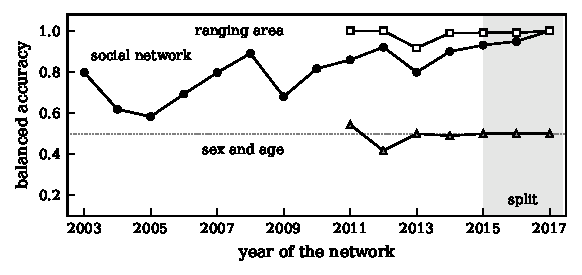
\includegraphics[width=\linewidth]{figs/fig-soc-ngogo.pdf}
\caption{\textbf{Ngogo: who went where.} Balanced accuracy with which each year's data
predict the group an individual joined after the split (gray band), from the social
network (vote of weighted neighbors), the ranging area (median GPS location, recorded
from 2011), and sex and age. Years with at least twenty labeled individuals. Dotted line,
chance.}
\label{fig:soc-ngogo}
\end{figure}

The network predicted the split years in advance (Fig.~\ref{fig:soc-ngogo}). In
2011--2014 the leading eigenvector of the normalized Laplacian assigned $86\%$ of
individuals to their later group, against $56\%$ for permuted labels. A vote of each
individual's weighted neighbors did better still, and the signal is present from
2007--2008, seven years before the community polarized. Sex and age predicted nothing in
any year. The network cut also separated the future groups \emph{within} males and
within females, so the fission line ran across the two attributes that primate homophily
studies use most, not along them.

The ranging area predicted the split better than the network: the median GPS location of
an individual assigned it to its later group without error from 2011, when the GPS
record begins. That raises the question whether the network carried any information
beyond shared space. Pairs of individuals with the same home-range overlap, the same
distance between ranging centers and the same sex combination answer it: at equal space,
future groupmates groomed each other no more than pairs that would end up on opposite
sides, with the difference in log grooming weight consistent with zero. The Ngogo
community divided along spatial neighborhoods that had existed for years, and its social
ties followed those neighborhoods.

The fission is therefore not homophilous in any measured trait, and it is not evidence
for locality either. It is spatial. Space and the network were already aligned when the
GPS record began, and no record of Ngogo shows which came first.

\section{Support follows the genealogy}

Three public whole-community networks from small-scale human societies carry individual
attributes or proximity: material support among $108$ adults of the Mayangna community of
Arang Dak, Nicaragua \citep{koster2018}; gift choices in a sharing game across eighteen
Agta forager camps in the Philippines \citep{smith2018agta}; and friendship nominations
with proximity in two Hadza camps in Tanzania \citep{fedurek2024}. For each, held-out ties
were predicted from attributes, from the network's own structure --- degree and closure
through shared partners, recomputed from training ties only --- and from both.

At Arang Dak the network's own structure predicts support better than the attributes
(sex, age, wealth, genetic and affinal relatedness, distance between households), with
AUC $0.83$ against $0.75$, and the two together reach $0.85$. Kinship is the largest
attribute effect. But kinship enters a model in two ways. As an attribute it is the
pairwise relatedness $r_{ij}$. As a network it is the genealogy, and the genealogy has
structure of its own: the number of kin two people share, and their distance in the kin
graph. That structure predicts support beyond pairwise relatedness, and it does so in
every one of $25$ cross-validation folds. Once the genealogy is in the model, closure in
the support network adds almost nothing. Support flows along the kinship network, to the
kin of one's kin and not only to close relatives. The community's weak block structure
aligns with blocks of the kinship graph, not with sex, age or space.

Among the Agta, gifts are barely predicted by exogenous attributes, whereas the network's own
structure reaches AUC $0.78$; but the camps have between seven and thirty-nine members,
far below $r_\kappa$, so their block structure is uninformative by the result of the
previous section. Among the Hadza, proximity and closure among friends both predict
friendship.

The genealogy is the case where the two mechanisms are hardest to pull apart, because it
is both at once. Descent and marriage are local rules --- a child attaches to its
parents, a spouse joins a family --- and the genealogy they grow is the substrate on which
kin homophily is usually defined. What the Arang Dak data establish is that support
follows the structure of that network, the paths through it, beyond the pairwise
similarity that a homophily model would assign. They do not exclude homophily on traits
that were never measured.

\section{Kinship and culture in prehistoric Europe}

Ancient genomes now reveal who was related to whom across millennia. Networks of
identity-by-descent (IBD) sharing among $705$ individuals buried in Central Europe between
the Neolithic and the Iron Age \citep{ringbauer2024,mallick2024}, a tie being at least one
shared segment of $12$ centimorgans or more, can be set against the archaeological culture
of each burial. Two individuals of the same culture are $2.6$ times more likely to share
IBD than two of different cultures at the same distance and in the same period. Spatially
contiguous partitions of the landscape with the same number of classes produce a ratio of
$1.3$, so genetic ties and material culture are coupled beyond geography.

The coupling is expected under both mechanisms: if similar groups exchanged partners, and
if groups linked by marriage came to share material culture. Only the order in time can
separate them, and at present sampling the order is not identifiable. A cross-lagged
design --- past kinship density predicting present shared culture, against past shared
culture predicting present kinship --- found a network-first effect that exceeded
distance-decay and permutation nulls but not a rewiring that preserves degrees and edge
lengths, and the effect rested on a single cultural transition. The coupling is real; its
direction waits for denser genomic sampling.

\section{An arrow of time}

The test that the synthetic societies single out is temporal: do ties come before
similarity? The Chaco region of the North American Southwest offers a rare record of it.
Ceramic assemblages from $280$ settlements, dated in $50$-year slices between AD~800 and
1300 \citep{mills2018,daems2023}, allow the similarity of every pair of settlements to be
followed through the rise and decline of the Chaco system, while the number of occupied
settlements grows from a few dozen to nearly two hundred and shrinks again. At each time
slice $t$ the settlements form a network by ceramic similarity, and the block model
partitions it into communities.

\begin{calculation}{forward and reversed convergence}
Let $s_t$ be the Brainerd--Robinson similarity of the ware proportions of two settlements
in slice $t$, and $\mathrm{same}_t$ the indicator that they share a community. For a pair
of slices $t<t'$ and the settlements present in both, the forward regression
\begin{equation}
  s_{t'}-s_t \sim \beta_{\rightarrow}\,\mathrm{same}_t + s_t + \text{controls}
  \label{eq:soc-fwd}
\end{equation}
measures the convergence effect $\beta_{\rightarrow}$: how much more similar two
settlements become if they shared a community, given how similar they already were. The
controls are distance decile and region. The time-reversed regression
\begin{equation}
  s_{t}-s_{t'} \sim \beta_{\leftarrow}\,\mathrm{same}_{t'} + s_{t'} + \text{controls}
  \label{eq:soc-bwd}
\end{equation}
asks the same question with the arrow turned around, and the forward excess is
$\beta_{\rightarrow}-\beta_{\leftarrow}$.

The reason to compute both is regression to the mean. A pair that shares a community is
selected for high similarity, and noise alone makes high values fall back, in either
direction of time. If the community structure is stationary --- each settlement's
composition fixed, with only sampling varying --- the two directions are statistically
equivalent and the expected forward excess is zero. A positive forward excess is a
direction of time in the record. The stationary null makes this exact: in each draw every
slice is redrawn multinomially from each settlement's pooled composition at the observed
sample sizes, re-partitioned, and evaluated on all intervals at once, so that overlapping
intervals stay as dependent as they are in the data.
\end{calculation}

\begin{figure}[!ht]
\centering
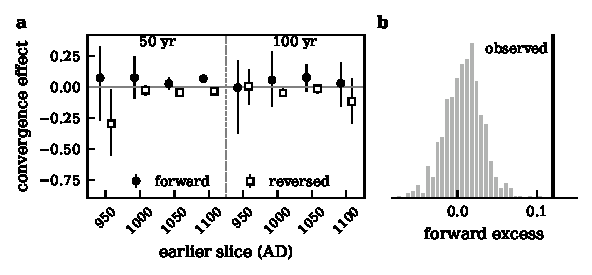
\includegraphics[width=\linewidth]{figs/fig-soc-chaco.pdf}
\caption{\textbf{An arrow of time in the Chaco record.} (a) Convergence effect for each
pair of slices, forward ($\beta_{\rightarrow}$, Eq.~\eqref{eq:soc-fwd}) and time-reversed
($\beta_{\leftarrow}$, Eq.~\eqref{eq:soc-bwd}), for intervals of $50$ and $100$ years
with at least thirty settlements in common. Bars, $95\%$ node-bootstrap intervals.
(b) Mean forward excess over the eight intervals (vertical line) against $500$
realizations of the stationary null (gray).}
\label{fig:soc-chaco}
\end{figure}

The two directions are not equivalent (Fig.~\ref{fig:soc-chaco}). Settlements that shared
a community converged over the following $50$ to $100$ years, beyond what geography
produces, while $\beta_{\leftarrow}$ was zero or negative in every interval. The mean
forward excess over the eight Chaco intervals exceeded every one of $500$ realizations of
the stationary null, $P<0.002$. It did so for consecutive slices and, separately, for
slices a century apart, which share no ceramic data and so cannot share sampling noise.
The forward excess is positive in nine of ten intervals across Chaco and the wider
Southwest \citep{mills2013}. No single interval survives a correction for multiple tests
on its own; the joint test was the one specified in advance.

If the convergence came from contact between adjacent villages, it would weaken with
distance inside a community. It does not: the interaction between shared membership and
distance is indistinguishable from the null. Convergence acted on the community as a
whole, over tens of kilometers, as expected for spreading through a connected network.

The converse arrow is present too. Similarity at one time predicts membership of the same
community at the next, beyond earlier membership, in seven of eight intervals. In the
language of the synthetic societies, the Chaco record shows contagion along the network
and homophily in the choice of partners, both at once.

\section{What the record says}

Across a primate community, three human communities, prehistoric genomes and an
archaeological time series, the traits most often invoked for homophily --- sex and age
--- organized neither the Ngogo fission nor human support ties. What did was structure:
spatial neighborhoods among the chimpanzees, the genealogy at Arang Dak, and in the Chaco
record the community structure of the exchange network, which preceded convergence in
material culture. Homophily was present as well: similar settlements later joined the
same community, and shared culture and genetic ties went together in prehistoric Europe.
Network structure often came first, and the two mechanisms acted together.

The limits are specific, and each names the data that would remove it. At Ngogo, space
and the network were aligned before the record began, and a pedigree would show whether
kinship drew the line both followed. At Arang Dak, the network that matters is the
genealogy, which is also the classic substrate of kin homophily; later survey waves would
give the Mayangna network a time axis. The Chaco communities are defined by ceramic
similarity, not by observed interaction, so a regional tradition whose clusters each
evolve as a unit would also converge forward; obsidian sourcing measures exchange
independently of style. Time-stamped proximity networks of forager camps with genealogies
\citep{migliano2017,dyble2015}, above $r_\kappa$ and with a time axis, would decide the
question at the scale this book predicts it should be decided.

\section{Summary}

Locality and homophily leave similar traces in a snapshot of a small society. Synthetic
societies with a known mixture of the two show which traces can be read. Dyadic models
that take a measured trait as given separate the mechanisms already at twenty
individuals. Comparing inferred communities with traits is weak at every size: locally
grown communities appear only above $r_\kappa$, and homophily blocks at realistic density
sit at an information threshold, Eq.~\eqref{eq:soc-detect}, that does not depend on size.
When traits spread along ties every snapshot statistic reverses, and only temporal order
identifies the mechanism.

The records agree with that map. The Ngogo fission followed neither sex nor age but the
spatial neighborhoods its network already traced. Support at Arang Dak followed the
structure of the genealogy beyond pairwise relatedness. Kinship and culture in prehistoric
Europe were coupled beyond geography, in an order the present sampling cannot resolve. And
the one record with a time axis, Chaco, has a direction: communities first, similarity
after, with similarity feeding back on later membership. Communities in these societies
are not simply the imprint of shared traits. Boundaries that the network draws can
accumulate differences --- in style, in kinship, in custom --- that homophily then
reinforces, which makes some of the diversity of early societies a consequence of their
network structure rather than only its cause.
